%!TEX root = ../../dissertation.tex


\section{Architecture} % (fold)
\label{sec:architecture}
This section presents the architecture of the system we propose as solution.

The system follows the architecture in Figure~\ref{fig:architecture1}.

A module in Racket was Build. This module provides a \gls{API} for the users to describe their models in the Racket Programming Language.
This \gls{API} is implemented in C++ using modern OpenGL. Each of these modules is explained in the following sections.

\begin{figure}[h!]
	\centering
	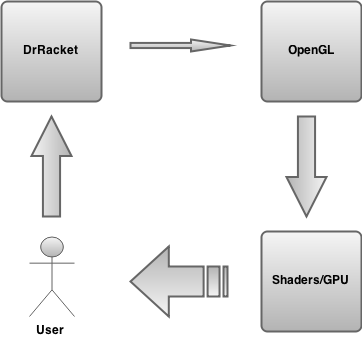
\includegraphics[width=0.55\textwidth]{images/Architecture/architecture1.png}
	\caption{Architecture Diagram}
	\label{fig:architecture1}
\end{figure}


\begin{figure}[h!]
	\centering
	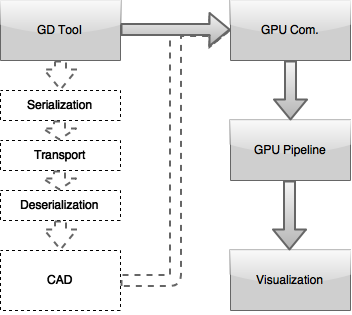
\includegraphics[width=0.55\textwidth]{images/Architecture/GD-Fast-Pipeline.png}
	\caption{Architecture Diagram}
	\label{fig:architecture2}
\end{figure}

\subsection{Racket API} % (fold)
\label{sub:racket_api}
Since the focus users for this system are architects and designers, which do not have large programming experience, several design decisions have been made taking this into account. The \gls{PL} that is used by the users is the Racket Programming Language. This is a \gls{PL} that was developed emphasizing pedagogy, is well known for being a good for beginners \cite{Findler1997}\cite{Findler2002}.
The racket module was build to allow the users to implement their models in the Racket Programming Language. 

% subsection racket_api (end)

\subsection{OpenGL Backend} % (fold)
\label{sub:opengl_backend}
We implemented the API with C++ using modern OpenGL. We use this platform with two main reasons, (1) OpenGL is a cross platform API for graphics, and (2) the previous experience with the platform.

% subsection opengl_backend (end)


% section architecture (end)
